\documentclass[aspectratio=169]{beamer}

\usetheme{default}
\usecolortheme{default}
\setbeamertemplate{navigation symbols}{}
\setbeamertemplate{footline}[frame number]

\usepackage[T1]{fontenc}
\usepackage[utf8]{inputenc}
\usepackage{lmodern}
\usepackage{graphicx}
\usepackage{tikz}
\usepackage[backend=biber]{biblatex}

\addbibresource{references.bib}

\setbeamercolor{background canvas}{bg=white}
\setbeamercolor{normal text}{fg=black,bg=white}
\setbeamercolor{frametitle}{fg=black,bg=white}
\setbeamercolor{title}{fg=black,bg=white}

\newcommand{\figureplaceholder}[1]{%
  \begin{tikzpicture}
    \draw[black!45, line width=0.8pt] (0,0) rectangle (0.98\linewidth,0.52\textheight);
    \node[text=black!60] at (0.49\linewidth,0.26\textheight) {#1};
  \end{tikzpicture}
}

\title{Questions on Correlated Uncertainties}
\author{}
\date{September 1, 2026}

\begin{document}

\begin{frame}
  \titlepage
\end{frame}

\begin{frame}{Main Questions}
  \begin{itemize}
    \item Quantify the effect of including correlated experimental uncertainties in the likelihood on the posterior distribution.
    \item Search for inference methods capable of estimating correlated experimental uncertainties from data.
  \end{itemize}
\end{frame}

\begin{frame}
  \centering
  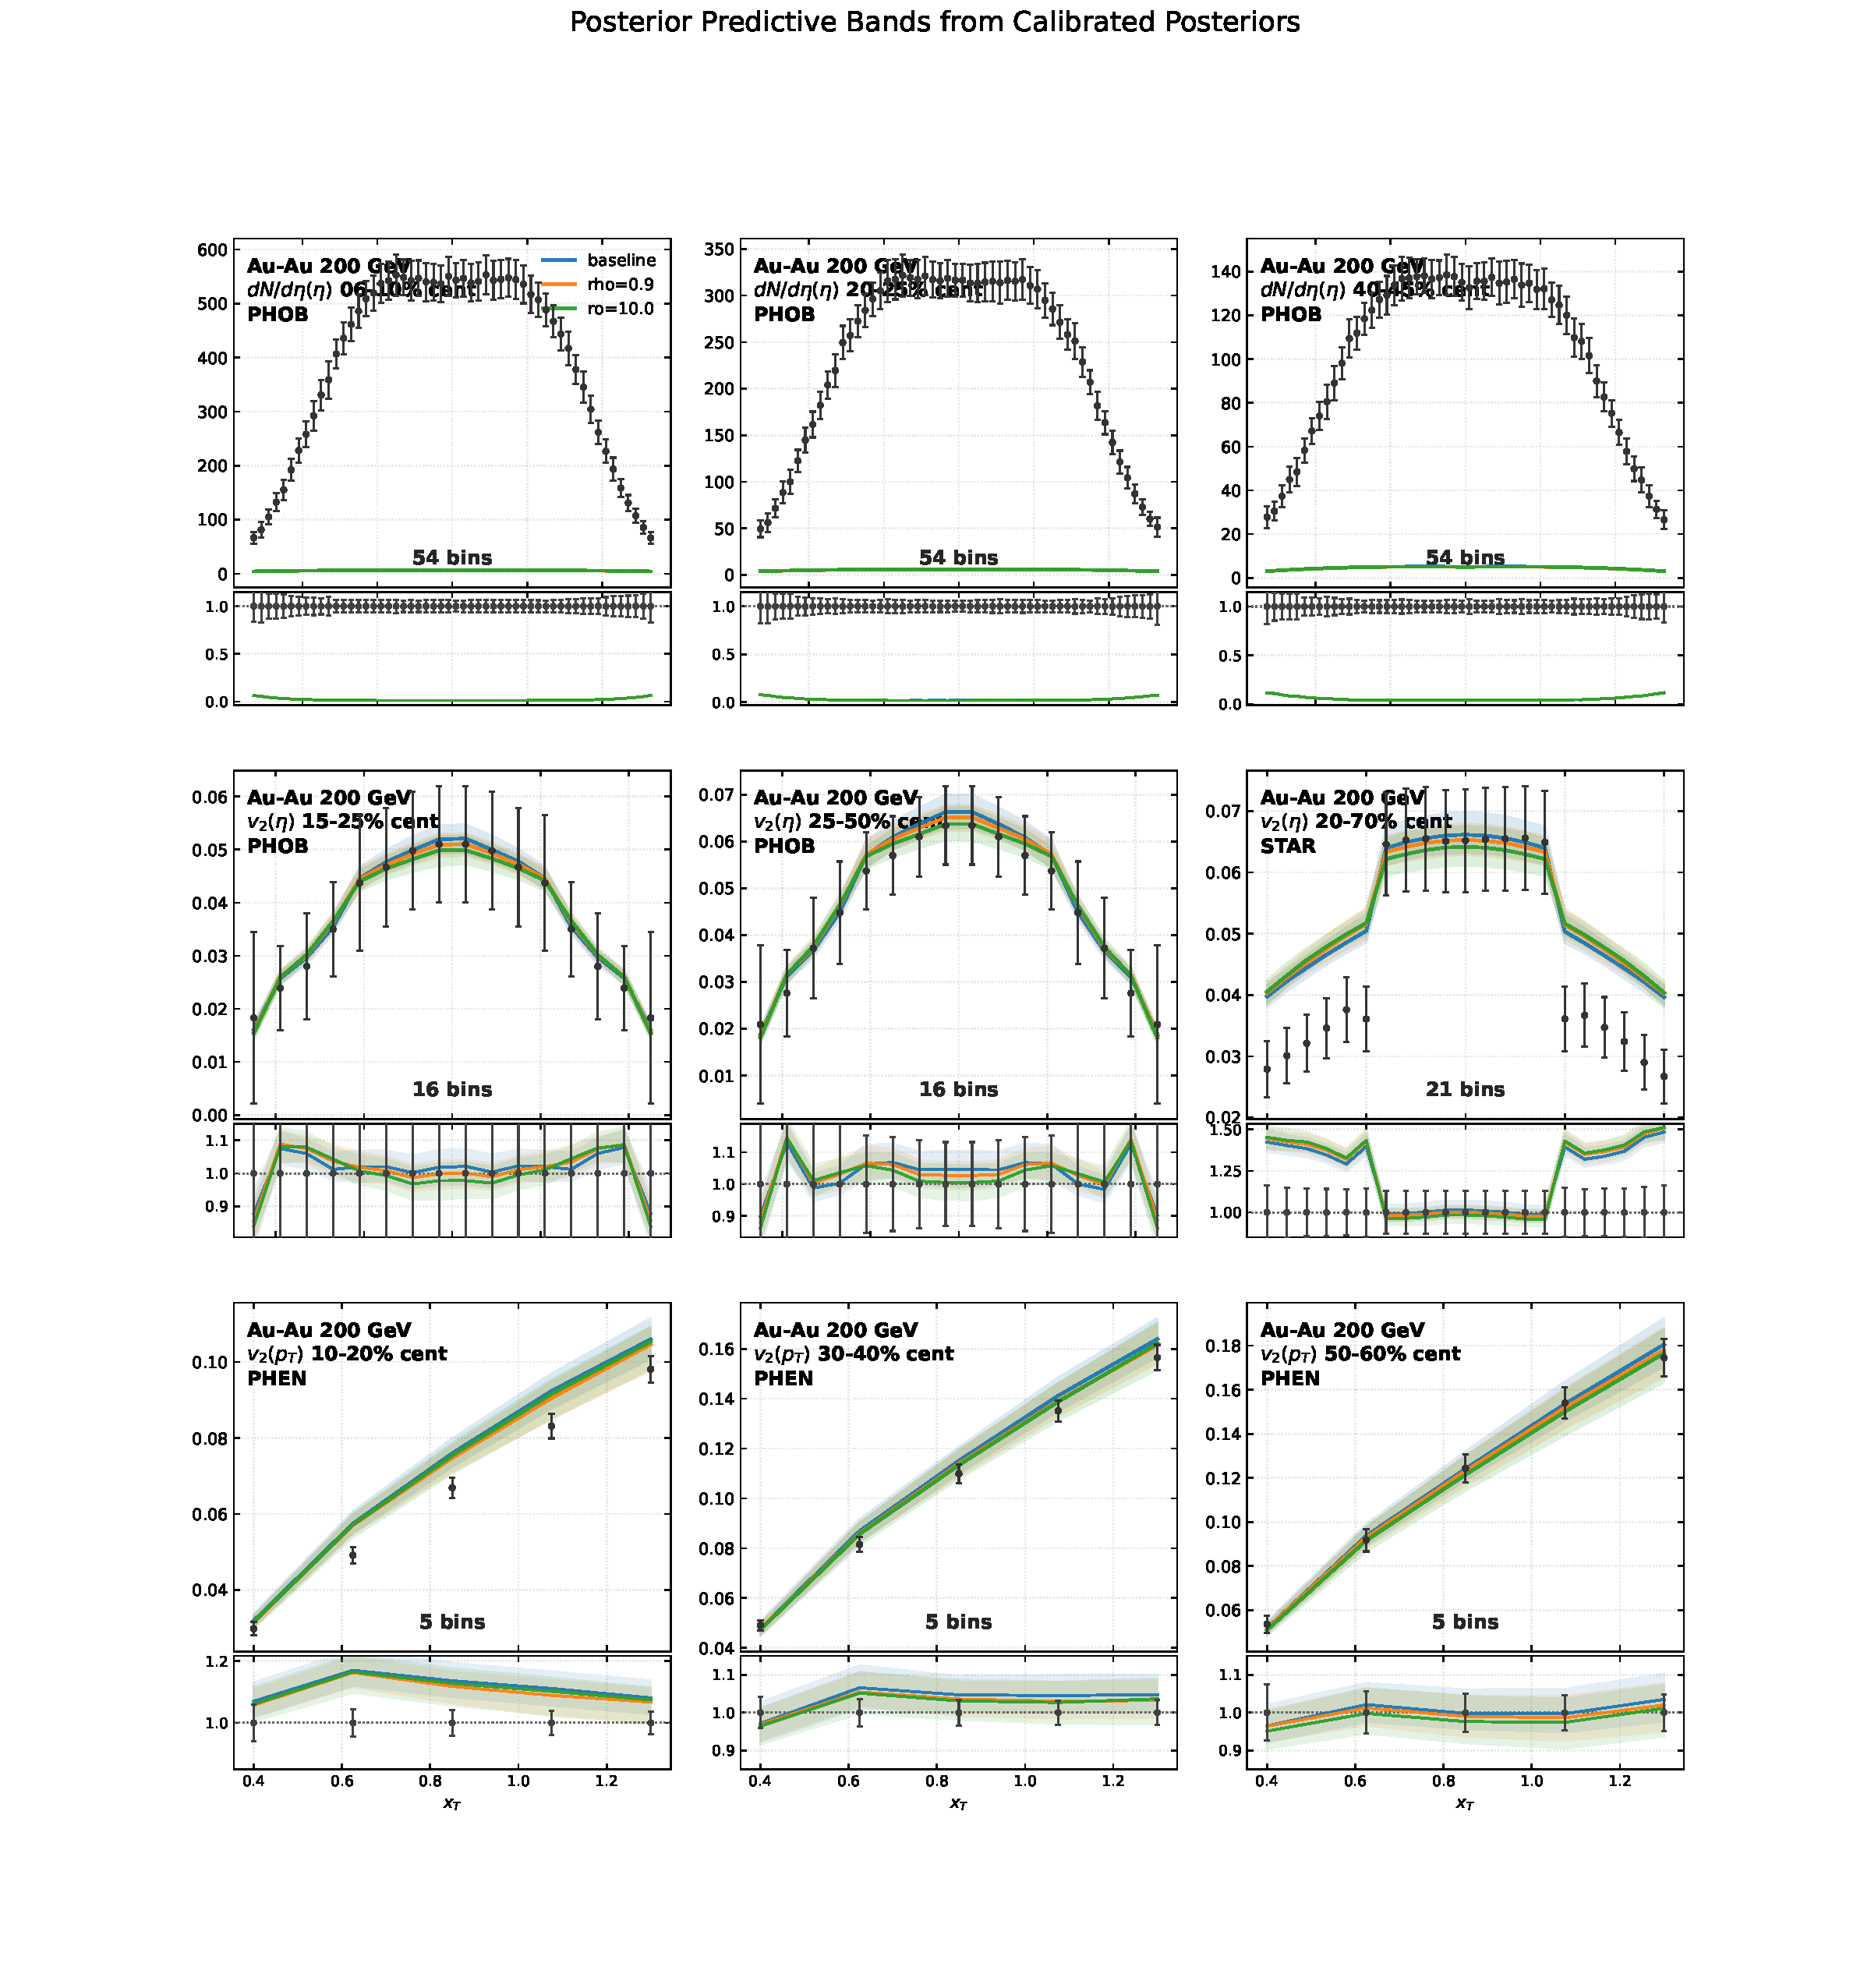
\includegraphics[width=1.06\textwidth,height=0.90\textheight,keepaspectratio]{img/posterior.pdf}
  \vspace{0.15cm}

  {\footnotesize Posterior distributions obtained with and without correlated uncertainty information in the likelihood.}
\end{frame}

\begin{frame}
  \centering
  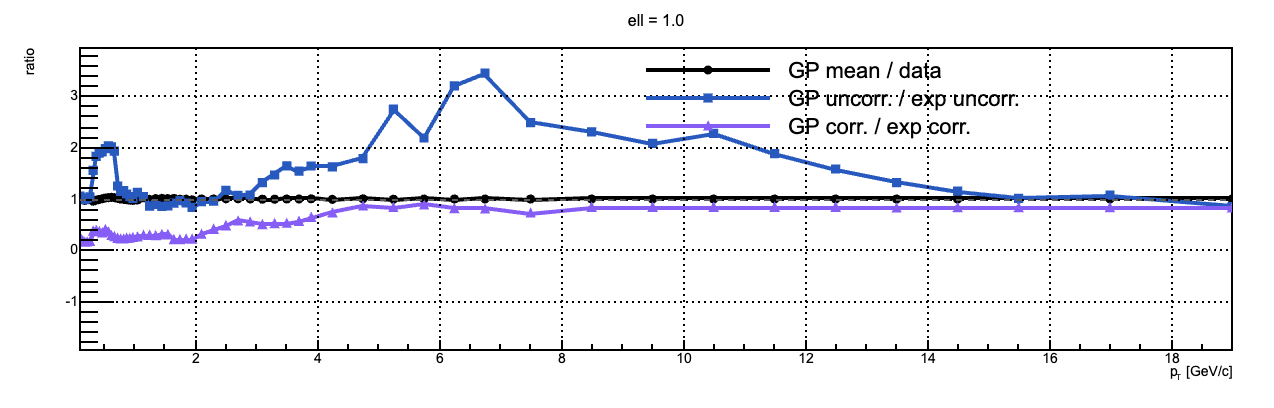
\includegraphics[width=1.06\textwidth,height=0.90\textheight,keepaspectratio]{img/Atlas-ell-1.0.png}
  \vspace{0.15cm}

  {\footnotesize Experimental correlated uncertainty fit through Gaussian Process.}
\end{frame}

\end{document}
